% !TEX root = ./main.tex
\section{Immediate implications of cosmic ray observations}
\label{sec:implications}

\subsection{Efficiency of particle acceleration in Galactic sources}

In the previous sections, we have discussed how the abundances of certain elements such as boron, lithium and beryllium in CRs provide us with valuable estimates of the time $\tau_{\rm esc}$ that CRs spend in the Galaxy before escaping.
%
Now, we delve deeper into the implications of these observations, specifically focusing on the energetic budget required by galactic sources to sustain the CR population.

Having in mind acceleration mechanisms similar to DSA, to describe the injection spectrum of protons, we assume a power-law form in momentum that accounts for both relativistic and non-relativistic particles:
%
\begin{equation}
N(p) = N_0 \left(\frac{p}{m c}\right)^{-\gamma} \, , 
\end{equation}
%
where $\gamma \gtrsim 4$. The normalization of $N(p)$ is determined by the condition that the integrated energy in particles matches the energy released in CRs by a single event:
%
\begin{equation}
4 \pi \int_0^\infty dp \, p^2 N(p) T(p) = E_{\rm CR}
\end{equation}

Solving for $N_0$, we find
%
\begin{equation}
N_0 = \frac{E_{\rm CR}}{4 \pi c (m c)^4 I(\gamma)},
\end{equation}
where $I(\gamma) = \int_0^\infty dx \, x^{2-\gamma} \left[ \sqrt{x^2+1} - 1 \right]$.

Note that due to spectral index values larger than 4, the total energy budget is determined by protons with energies of $\sim$GeV, and we can ignore the existence of minimum and maximum momentum.

Assuming high energies where ionization losses can be neglected and solar modulation has no significant effect, the proton spectrum contributed by identical sources occurring at a rate $\mathcal R$ can be expressed as:
%
\begin{equation}
f_{\rm p}(p) = \frac{E_{\rm CR} \mathcal R}{8 \pi^2 R_{\rm d}^2 c (m c)^4 I(\gamma)} \left( \frac{p}{mc}\right)^{-\gamma} \frac{H}{D(p)},
\end{equation}

Using the definition of intensity, given in appendix~\ref{app:intensity}, and considering that in the relativistic limit $E \simeq p c$, we obtain:
%
\begin{equation}
I_{\rm p}(E) = \frac{E_{\rm CR} \mathcal R c}{8 \pi^2 R_{\rm d}^2 (m c^2)^2 I(\gamma)} \left( \frac{E}{mc^2}\right)^{2-\gamma} \frac{H}{D(E)}
\end{equation}
%
which gives for $E = 10$~GeV:
%
\begin{equation}
E^2 I_{\rm p}(E) \simeq 2 \times 10^3 \left(\frac{E_{\rm CR} \mathcal R}{10^{40} \, \text{erg} \, \text{s}^{-1}}\right) \, \text{GeV} \, \text{m}^{-2} \, \text{s}^{-1} \, \text{sr}^{-1}
\end{equation}

\begin{figure}[t]
\centering
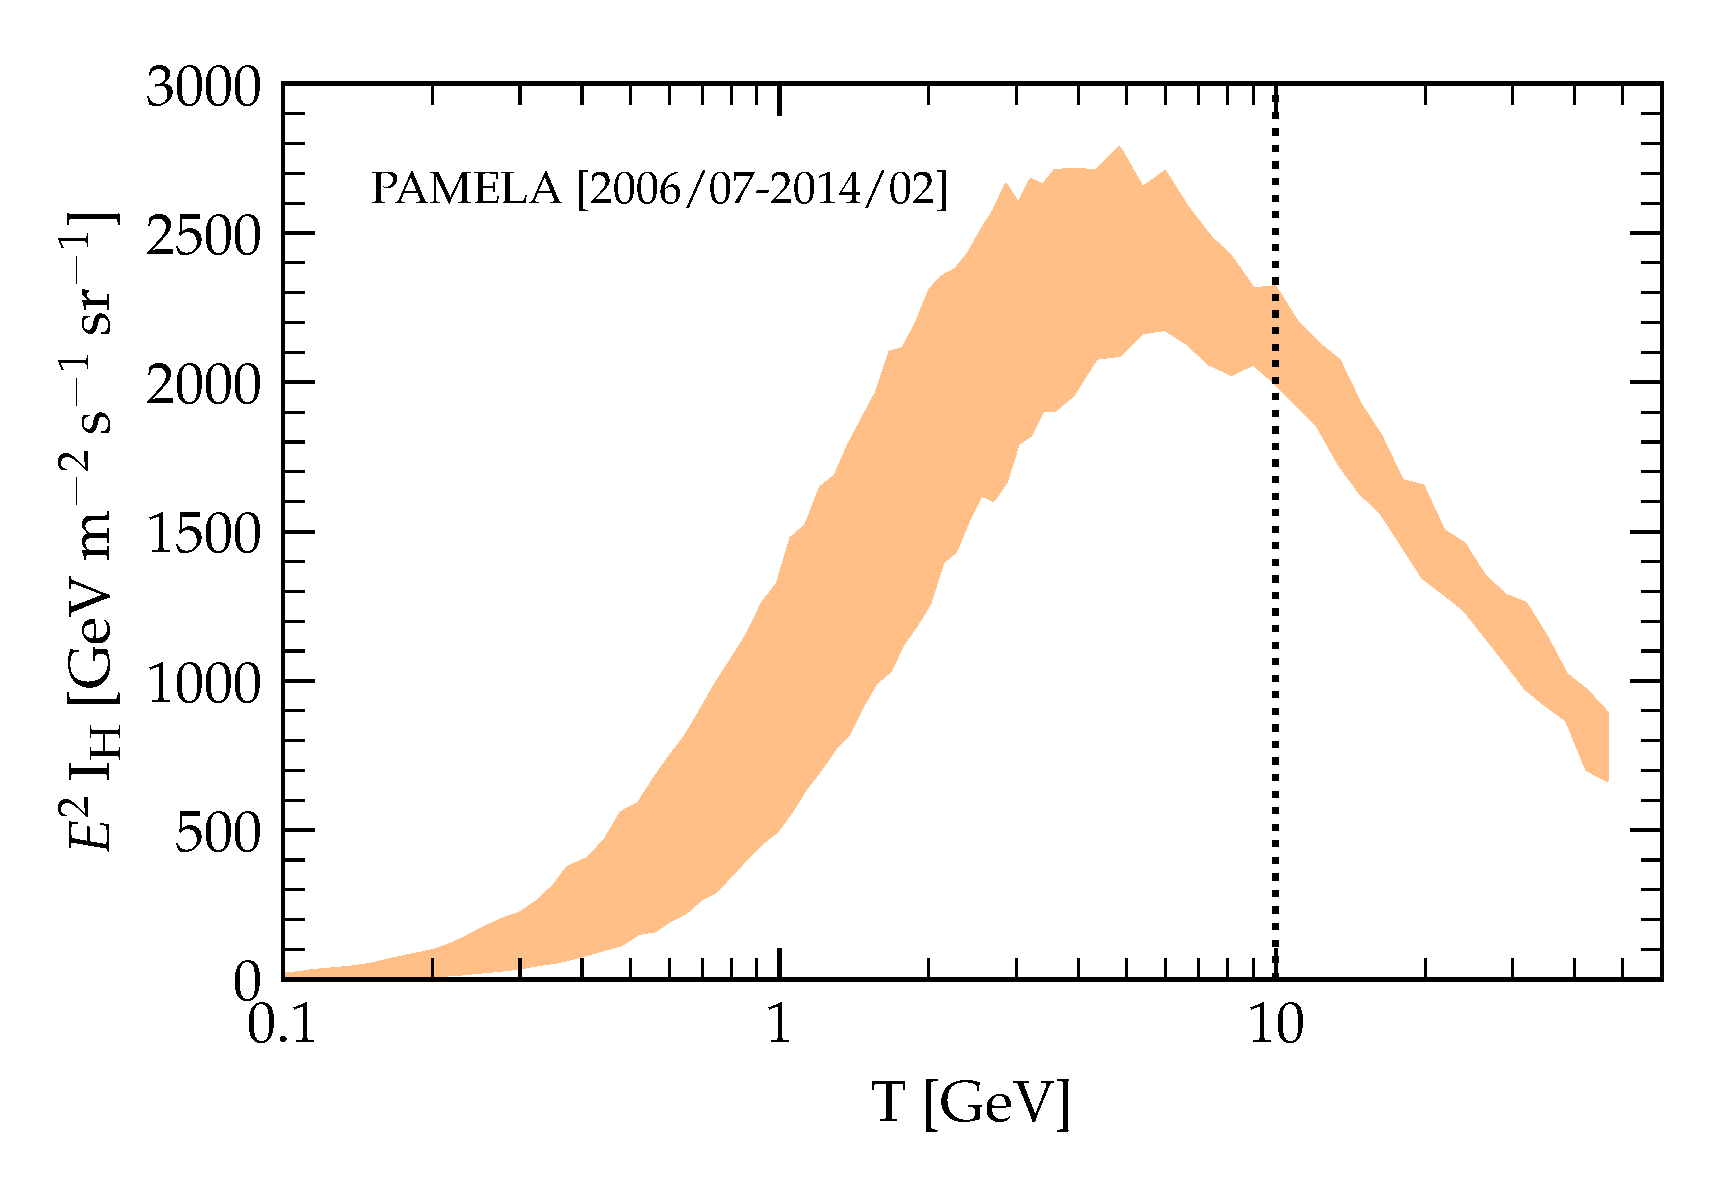
\includegraphics[width=0.6\textwidth]{figures/protons_le.pdf}
\caption{The proton intensity measured by the PAMELA experiment over a large fraction of the Solar activity cycle ~\cite{PAMELA.2011.proton}.}
\label{fig:pamelaprotons}
\end{figure}

By comparing this equation with the proton flux measured by the PAMELA experiment, as shown in figure~\ref{fig:pamelaprotons}, we find that in order to maintain a steady-state, the power that Galactic sources inject into the Galaxy in the form of CR protons needs to be approximately $\mathcal L \simeq E_{\rm CR} \mathcal R \simeq 10^{40} \text{erg} \, \text{s}^{-1}$ for a time not smaller than $\tau_{\rm esc}$.

Assuming that CRs are produced by supernova explosions with a rate of about 2 per century and with a typical mechanical energy release of $10^{51}$ erg per explosion, the luminosity amounts to $6 \times 10^{41}$ erg/s, significantly exceeding the required one. Hence, it is necessary to invoke an efficiency of a few percent in the conversion between supernova kinetic energy and CR energy to make this hypothesis viable.

Detailed calculations provide a more accurate estimate of the total acceleration efficiency, typically ranging from 5\% to 10\% (including nuclei), for the majority of supernova remnants. This efficiency is well described in recent models of diffusive shock acceleration~\cite{Morlino2017hsn}, upraising the hypothesis that CRs acquire their energy from Galactic stellar explosions to the rank of a \emph{paradigm}.

Over the years, alternative sources of energy, such as those in the Galactic Center region, star clusters, or OB associations\footnote{OB associations consist largely of very young, massive stars (about 10 to 50 solar masses) of spectral types O and B.}, have been proposed to explain galactic CRs. 
%
Interestingly, the star clusters scenario for the origin of galactic CRs have recently gained renewed attention based on gamma-ray observations (see S.~Gabici's lecture notes in this volume).

%%% SI PUO STIMARE L'EFFICIENZA IN SNE, vedi Morlino review.

\subsection{Constraints on the microphysics of galactic transport}

In the previous sections, we have discussed how the remarkable longevity of CRs, which greatly exceed the time it would take them to propagate freely at the speed of light, suggests that CRs undergo a random walk, continually scattered as they traverse their path from the sources to Earth.
%
Furthermore, the absence of a strong anisotropy, $\mathcal{O}(1)$, toward the galactic center for CRs with energies below $10^{15}$ eV implies that multiple scatterings wash out the anisotropy that would be expected if there were no scattering~\cite{Hillas2005jpg}. 

The scattering cannot be attributed to ISM nuclei, as the mean free path for Coulomb collisions of relativistic nucleons in the dilute ISM, given by $\lambda \simeq \frac{1}{n_{\rm H} \sigma_{\rm T}} \sim 10^{24}$ cm, is far too long.

Hence, the most likely scattering mechanism is the interaction of CRs with plasma waves, which are fluctuating electromagnetic fields in the ISM. The presence of a random component of the Galactic magnetic field is inferred from fluctuations in rotation measures, combined with estimates of thermal electron density and synchrotron depolarization. Recent analyses have reported a strength of this component at around $1-3 \mu$G~\cite{Ferriere2023epj}.

Understanding the production of these plasma waves and their influence on the dynamics of CR particles is a crucial topic in the theoretical investigation of CR physics.

Typically, the energy spectrum of the turbulent field is assumed to follow a power-law distribution with an outer scale of $L \sim 10$ pc, where energy is injected. This energy then cascades down to smaller scales until it dissipates at the dissipation scale.

For CR nuclei in the GeV-TeV energy range and charge $Z$, the Larmor radius in this magnetic field is given by:
%
\begin{equation}
r_{\rm L} \simeq 10^{-5} \, \text{pc} \left( \frac{E / Z}{10 \, \text{GeV}} \right) \left( \frac{B}{\mu\text{G}}\right)^{-1}  
\end{equation}

This length scale is much smaller than the random field injection scale but larger than the dissipation scale. Consequently, a CR nucleus is expected to encounter numerous magnetic scattering centers before reaching Earth.

This transport mechanism is understood in terms of resonant wave-particle interaction, where CRs primarily scatter off waves with wavelengths comparable to their gyroradius. 

Under these conditions, a particle interacts with a wave remaining in phase with the wave over many cycles. 
%
This scattering leads to an effective diffusion in pitch angle which, in turn, regulates their diffusion in real space.

The resonant condition can be expressed as
%
\begin{equation}
k_{\rm res} = \frac{1}{\mu r_{\rm L}}
\end{equation}
%
where $k_{\rm res}$ represents the wavelength of the \emph{resonant} magnetic perturbation and $\mu$ is the cosine of the particle's pitch angle.

Within quasilinear theory the spatial diffusion coefficient results from the pitch-angle-cosine $\mu$ average of the inverse of the pitch-angle diffusion coefficient $D_{\mu\mu}$ (see appendix~\ref{app:diffusioncoefficient}):
%
\begin{equation}
D \simeq \frac{(1-\mu^2) v^2}{D_{\mu\mu}}
\label{eq:dandbasta}
\end{equation}

The pitch-angle diffusion rate must depend upon the distribution of wave energy, and in weakly turbulent magnetic fields, we obtain:
%
\begin{equation}
D_{\mu\mu} \simeq \pi \Omega (1-\mu^2) k_{\rm res} \mathcal F(k_{\rm res})
\label{eq:dmumusimeq}
\end{equation}
%
where $\Omega = c / r_{\rm L}$ is the gyrofrequency, and $\mathcal F$ is the power in modes of wavenumber $k_{\rm res}$ normalized such that its integral gives the fraction of energy density in the turbulent components with respect to the regular field:
%
\begin{equation}
\int_{1/L}^\infty \! dk \, \mathcal F(k) = \frac{\langle \delta B^2 \rangle}{B_0^2}
\end{equation}

Intuitively, if we associate the angle by which the fieldlines are bent $\delta B/B_0$ with the scattering angle $\delta \theta$, and assume the particles encounter uncorrelated waves at frequency $\Omega$, then the angular diffusion coefficient is $\langle (\delta \theta)^2 \rangle / \delta t \sim \Omega (\delta B/B_0)^2$ which is essentially equation~\eqref{eq:dmumusimeq}. 

Combined with equation~\eqref{eq:dandbasta} the diffusion coefficient reads
%
\begin{equation}
D \simeq \frac{1}{3} r_{\rm L} c \frac{1}{k_{\rm res} \mathcal F(k_{\rm res})}
\label{eq:dzz}
\end{equation} 

We recall now from equation~\eqref{eq:grammage} that the best fit to secondary-over-primary CRs in the Galaxy indicates a diffusion coefficient of $D/H \sim 2$ for particles around 10 GeV, where $D$ is measured in units of $10^{28}$ cm$^2$ s$^{-1}$ and $H$ represents the scale height in kpc. 
%
Combining this information with the determination of the halo size obtained from unstable species, $H \sim 5$ kpc, we obtain a \emph{measurement} of the normalization of the diffusion coefficient to be approximately $D \sim 10^{29}$ cm$^2$ s$^{-1}$.

%DIRE QUI DEL MFP? {\color{magenta}{Ti riferisci alla condizione che il mean free path deve essere molto piu' piccolo rispetto alle dimensioni di H? Sarebbe interessante dedicargli un paragrafetto}}

By inverting equation~\eqref{eq:dzz}, we can finally determine the required level of turbulence at the scale of 10 GeV particles in order to replenish the observed amount of secondary particles:
%
\begin{equation}
k_{\rm res} \mathcal F(k_{\rm res}) \simeq \text{few} \times 10^{-6}
\end{equation}

In summary, even such a small perturbation at a scale corresponding to the size of the solar system, $\sim$A.U., is enough to significantly extend the transport time of CRs in the Galaxy from thousands of years to millions of years!

